%%%%%%%%%%%%%%%%%%%%%%%%%
%%%
%%% Chapter - Conclusion
%%%
%%%%%%%%%%%%%%%%%%%%%%%%%
\chapter{Conclusion}
\label{ch:conclusion}
In this dissertation, we explored haptic experience design (\haxd), looking at its process to inform how to design, build, and evaluate \haxd support tools.
%We leave the specific findings from each of our studies as best articulated in their respective chapters.
In this chapter, we summarize our research contributions from the preceding chapters and provide final thoughts about the \haxd process and support tools.
In particular, we discuss process, including challenges and strategies haptic designers can use to overcome those challenges, and
findings with specific implications for designing and developing software tools to support \haxd.
We conclude with directions for future work and final remarks on supporting \haxd.

\osE{Only so much can be done in the scope of a PhD dissertation, and so we note that this is not a complete description of \haxd.}
\osE{Our case study approach gave us a balance of depth, breadth, and grounded information; our selections for each information source necessarily shape our findings.}


%%%%%%%%%%%%%%%%%%
%
% Section - Description of the HaXD Process
%
%%%%%%%%%%%%%%%%%%
\section{Summary of Research Findings}
We summarize our more specific findings organized by approach: depth, breadth, and grounded capstone.


\begin{figure}[htbp]
\begin{center}
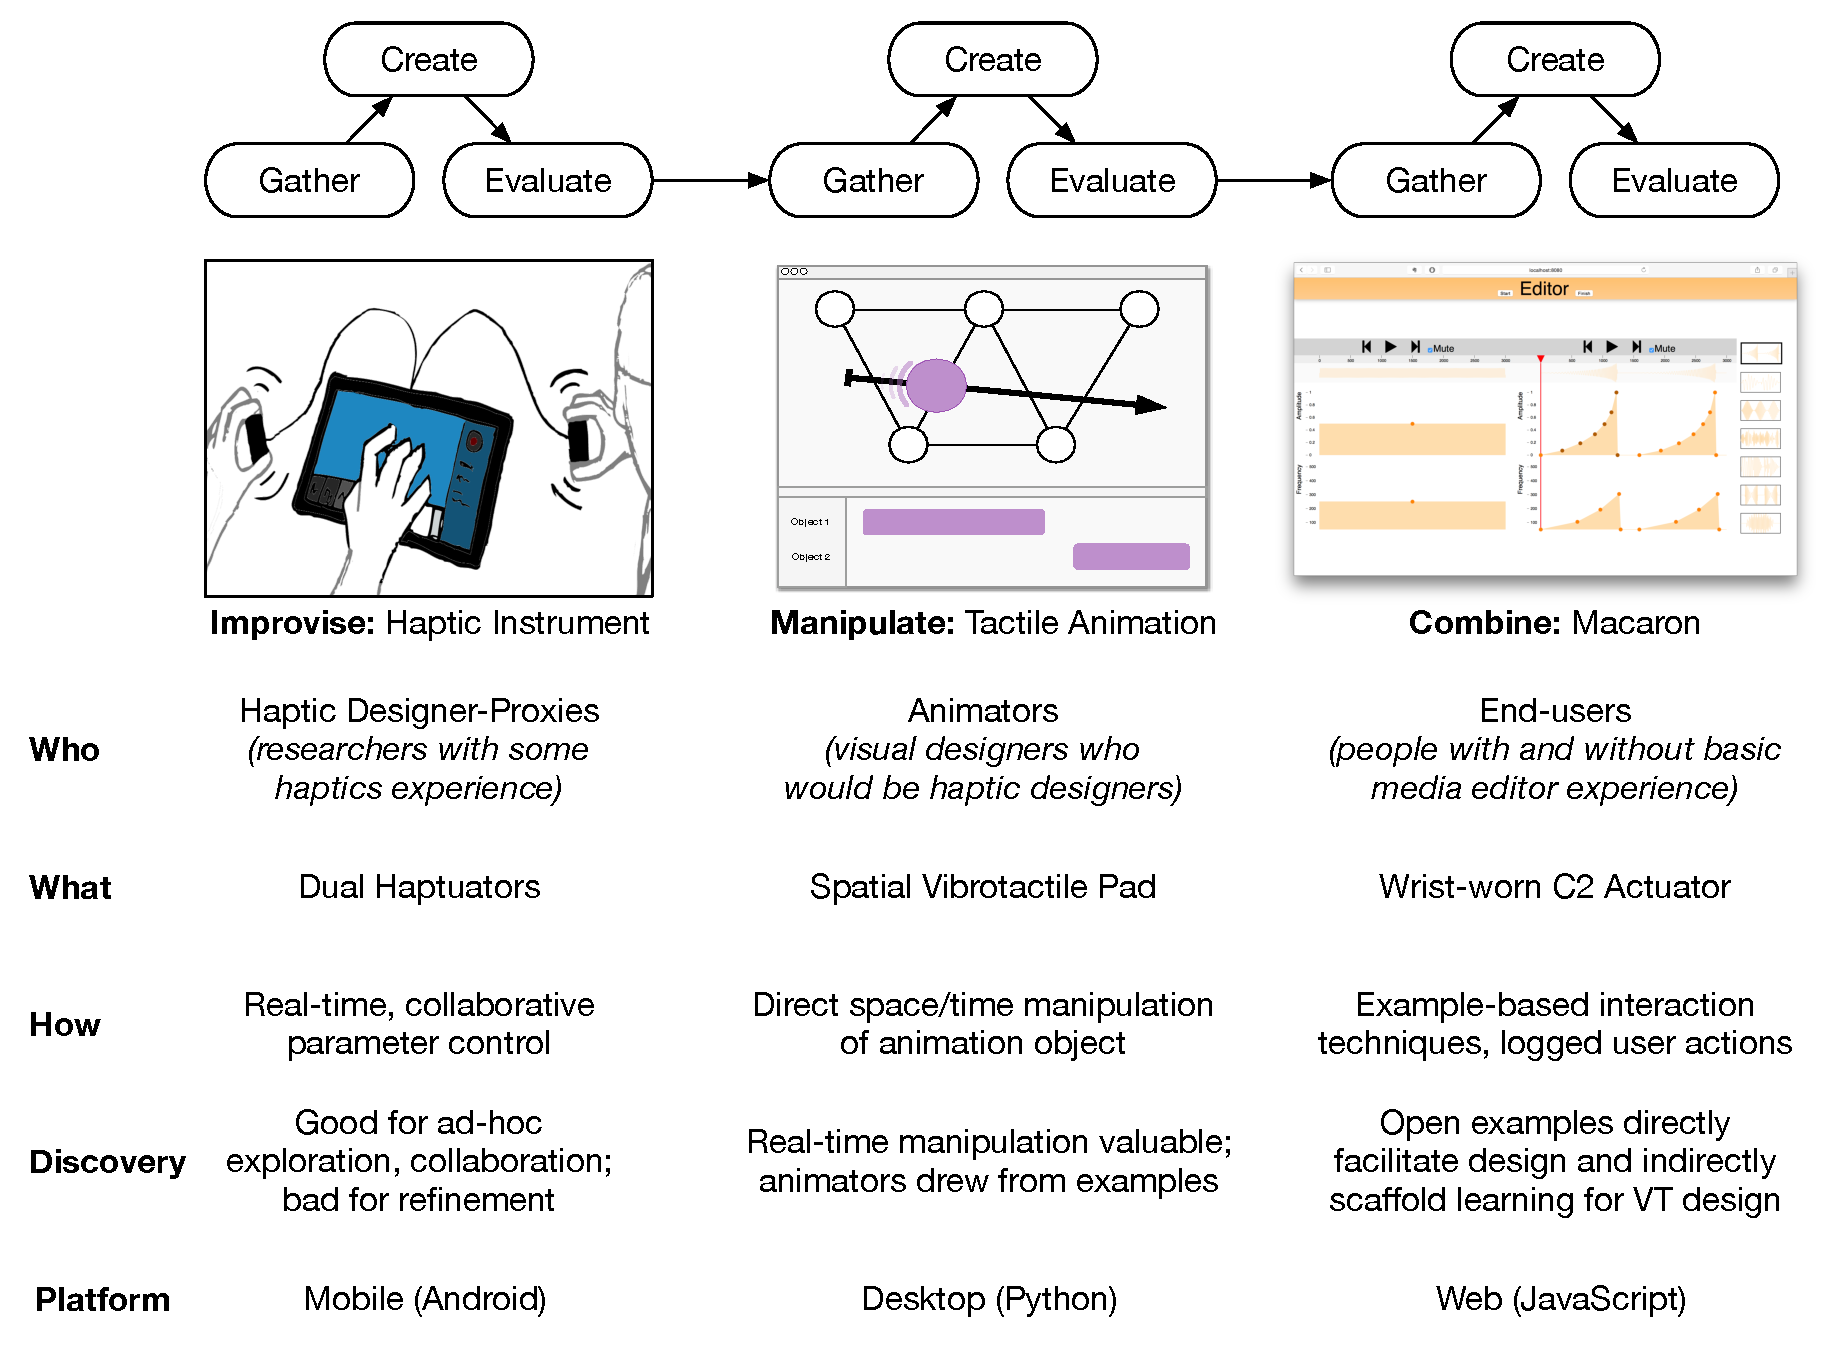
\includegraphics[width=\textwidth]{HaXDTheoryCaseStudyOutline-2016-08-11}
\caption{Vibrotactile design case studies. Each studied an aspect of vibrotactile design with a varied set of users, devices, platforms, and foci.}
\label{fig:intro:casestudyoverview}
\end{center}
\end{figure}



\subsection{Depth: Vibrotactile Design Tool Case Studies}
Through Chapters \ref{ch:hapticinstrument}-\ref{ch:macaron} we designed, built, and studied a trio of \haxd support tools.
Each case study investigated a different set of design concepts with varying user populations, VT devices, and design challenges (\autoref{fig:intro:casestudyoverview}).
%Each followed three design steps: \emph{gather}, finding requirements and previous design elements; \emph{create}, where we design and build the tool; and \emph{evaluate}, where we test the tool with its target population and consolidate lessons learned.
We include HapTurk (\autoref{ch:hapturk}), a VT \emph{sharing} technique, in this discussion.
We began with an initial hypothesis: that real-time feedback and collaboration could improve the haptic design process.
Through our tools, this hypothesis was confirmed, elaborated, and refined.

\inlineHeading{Initial Exploration: The Haptic Instrument (\autoref{ch:hapticinstrument})}
In Study 1, the Haptic Instrument, we focus on real-time, rapid design of VT sensations with a first look into themes of real-time design and collaboration.
%When participants worked with our tool, mHIVE, compositions couldn't be edited, suggesting mHIVE was suitable for exploration and improvised communication, but not as suited to refining ideas.
%We also found informal, collocated collaboration useful, but leave future examination of collaboration support to side projects (described next in \autoref{ch:intro:approach:breadth}).
Our implemented haptic instrument, mHIVE, showed us that rapid exploration was possible with real-time feedback, demonstrated value in informal, collocated collaboration, and gave evidence that showing rather than telling about haptic sensations could circumvent an impoverished language (\eg, what do you think of \emph{that}).
 mHIVE also showed us that there are distinct roles to be played by different tools: mHIVE was successful for early \emph{sketching}, but did not enable \emph{refining} and had a learning curve.


\inlineHeading{Direct Manipulation Pipeline: Tactile Animation (\autoref{ch:tactileanimation})}
%In Study 2, Tactile Animation, we developed a single abstracted animation object directly manipulated in both space and time.
%In this study, we focused on building a usable tool to support exploration and refinement, and investigate a generalized rendering pipeline in detail to understand how to build haptic design tools.
%Animators found our tactile animation tool, Mango, easy-to-use, and confirmed our findings about the value of real-time exploration.
%We also found that ``soft features", like copy/paste and undo/redo, were extremely important.
Our second tool, Mango, followed up on these themes with a focus on implementation.
We established a rendering pipeline for both design and playback.
A direct-manipulation metaphor let participants both \emph{sketch} in real-time and \emph{refine} their designs.
In addition, an animation paradigm enabled our visual animators to transfer their skills to tactile animation.
Our evaluation study found evidence for reuse: repetition played a large role in tactile animations, and participants again drew inspiration from their experience or external examples (\eg, a YouTube video of a heartbeat) - and noted the engagement of multimodal design, \eg, designing for an audio clip.
These both informed Macaron.


\inlineHeading{Example Use and Analytics: Macaron (\autoref{ch:macaron})}
%One stand-out result from both Mango and mHIVE is that designers drew from their experience or examples found in the world, and wanted to re-use what they had created (e.g., through copy and paste).
%In Study 3, we explore the role of examples in haptic design with a web-based tool, ``Macaron", a vibrotactile track-based editor with visible, incorporable examples directly embedded in the interface.
%Macaron was implemented using the understanding we gained from Study 2, giving us more opportunity to focus on capturing and studying the design process, especially using interaction logs to investigate example use.
%%This study is codenamed ``Project Macaron" and consists of two phases.
%%Phase I, ``algorithms and interaction techniques", builds a set of perceptually-verified ways to manipulate examples and incorporate them into designs.
%%In Phase II, we use the results of Phase I to create a haptic design gallery interface, and study how and when users incorporate examples into their VT designs.
%%In this way we hope to consolidate our findings from mHIVE and Mango, and capture our participants' design process more concretely through logging of user actions.
%We found examples were used primarily as templates to inform initial design, making each individual design easier but also scaffolding the user's understanding of how to create VT effects.
%%These studies are described in more detail in \autoref{ch:hapticinstrument},  \autoref{ch:tactileanimation}, and \autoref{ch:macaron}.
With our third tool, Macaron, we were able to easily implement the system (drawing from Mango's architecture), allowing us to study our participants' process more closely.
We found a number of concrete recommendations for \haxd tools, and confirmed the value of \emph{browsing} examples: we found different strategies for using examples in the initial design process, and open or visualized examples helped designers learn how to conduct VT design.
 Macaron also helped us find our more nuanced understanding of our initial hypotheses. Real-time feedback is useful as a preview, to get the right frequency, amplitude, or timing. However, participants would also step back to feel the entire design in its entirety, something that can be done

\inlineHeading{Feedback at Scale: HapTurk (\autoref{ch:hapturk})}
	%is a collaboration with PhD candidate Hasti Seifi on different techniques to crowdsource feedback on VT icons. Master's student Salma Kashani and undergraduate Matthew Chun are developing visualizations and low-fidelity VT icons during summer 2015.
	While not an iterative design tool study, HapTurk is a focused investigation of a VT design technique for collecting large-scale feedback on VT icons.
%	Haptic devices cannot be sent to hundreds or thousands of people for feedback, but collecting in-lab feedback can be expensive, and informal feedback from colleagues is limited in scope.
%	We investigate whether visual or low-fidelity \emph{proxies} can stand in for high-fidelity VT effects, with implications for both collecting feedback and broadcasting VT sensations more widely.	
	HapTurk (\autoref{ch:hapturk}) allowed us to study \osE{a specific piece of collaboration: how to widely transmit designs.}
	% collaboration more thoroughly, as we focused on other aspects of design with Mango and Macaron.
	We found that VT icons could be \emph{shared} over MTurk to elicit large-scale feedback from remote users.
	We also found affective qualities of VT icons could be communicated through proxies, suggesting we can express haptic ideas in different modalities.


\subsection{Breadth: Focused Haptic Design Projects}
\label{ch:conclusion:approach:breadth}
Together, mHIVE, Mango, and Macaron have informed us on both important features and roles for design tools, given us insight into implementation and evaluation, and helped us study \haxd as a process.
HapTurk extended this investigation to collaboration.
%To further our understanding, we conducted several focused projects which broadened our understanding of different devices and application areas.
To broaden our understanding of haptic design, we undertook several more focused haptic design projects to look at different activities, application areas, and haptic modalities.
In \textbf{\autoref{ch:applications}}, we described several smaller projects that gave opportunities for practicing haptic design and exploring other types of haptic feedback:

\inlineHeading{FeelCraft (\autoref{sec:applications:feelcraft})}  a plug-in architecture that augments media with customizable spatial VT effects.
	FeelCraft explored existing infrastructure for haptic media, and for designing VT effects for a popular video game, MineCraft.
	
\inlineHeading{Feel Messenger (\autoref{sec:applications:feelmessenger})} a chat program augmented with expressive, customizable VT effects using commodity hardware and APIs.
	
\inlineHeading{RoughSketch (\autoref{sec:applications:roughsketch})}  a painting application for the TPad Phone, a variable-friction mobile device, for the World Haptics 2015 Student Innovation Challenge. 
	Variable friction is a significant contrast to VT sensations as it is intrinsically connected to input: no sensation can be felt without active movement by the user.
	
\inlineHeading{HandsOn (\autoref{sec:applications:handson})} a conceptual model for creative education software using low-cost, DIY haptic hardware, giving us an understanding of how to work with 1-degree of freedom force feedback and an educational context.

\inlineHeading{CuddleBit (\autoref{sec:applications:cuddlebit})} a project inspired by the Haptic Creature \cite{Yohanan2011affectivetouch,Yohanan2011affectdisplay,Chang2010} and CuddleBot project \cite{Allen2015cuddlebot}.
	We use small, breathing robots to explore the display of emotion, and extend our findings from VT design tools into new tools for this modality: Voodle and MacaronBit.





\subsection{Ground: Data from Hapticians}
In \textbf{\autoref{ch:hapticianinterviews}}, we complement our design-based inquiry with data from haptic experience designers, or \osE{as we suggest calling them,} hapticians.
Haptic designers are difficult to access as they are both rare and often work in proprietary contexts, with limited ability to speak about their process.
To include hapticians' perspectives without severely hindering our design tool development, we conducted a grounded theory analysis of interviews with six haptic designers.
We characterized cross-cutting themes at three levels of scope: 1) the holistic nature of haptic experiences; 2) the collaborative ecosystem of haptic designers and related stakeholders; and 3) the larger cultural context of haptics in the public consciousness.
We augmented these interview findings with those from a workshop \osE{we} organized at a major international haptics conference, World Haptics 2015, which let us connect with designers more widely.

Our findings showed that haptic designers follow a general user-experience design process, but with added challenges because they work with haptics.
We articulated these challenges, \osE{gave} concrete recommendations on how to make progress on them, and finally gave a vision of haptic experience design as it might be practiced in the near future.
These results overlap with our findings from our design-based inquiry: some conclusions are confirmed, with similar themes emerging both from expert hapticians and our design studies; others emerged from only one source.


%%%%%%%%%%%%%%%%%%
%
% Section - Process/Requirements
%
%%%%%%%%%%%%%%%%%%
\section{\haxd Process: Requirements for Tools}
In this section, we examine our findings about the \haxd process. %, including challenges and strategies that designers can follow.
In \autoref{ch:hapticianinterviews}, we saw that haptic designers follow a familiar design process.
However, we also saw that there are unique challenges that differentiate \haxd from other modalities of design, which are confirmed by our work on \haxd support tools and our focused design projects.

We begin by discussing four design activities that occur generally in design, but need to be explicitly supported for \emph{sketch}, \emph{refine}, \haxd: \emph{browse}, \emph{share}.
Then, we comment on some approaches for handling the diverse devices and modalities employed by haptic technology.
After, we discuss some techniques to imbue haptic experiences with meaning and realism.
Finally, we talk about the importance of customization and how to support it.

%%%%%%%%%%%%%%%%%%
% SubSection - Description of the HaXD Process
%%%%%%%%%%%%%%%%%%
\subsection{Contextual Activities of Design: Sketch, Refine, Browse, Share}
In our first exploration of \haxd support tools, the Haptic Instrument (\autoref{ch:hapticinstrument}), we found evidence that mHIVE was able to support exploration and sketches of haptic ideas, but not refinement into final designs.
mHIVE was also able to support collaboration in certain ways.
In our followup studies, we explored these activities that draw upon a designer's context, eventually arriving at four that we found are valuable when thinking about tool design: browsing examples, sketching new ideas, refining existing ideas, and sharing ideas with others (\autoref{tab:designactivities}).
These activities can occur at any point in the design process, and we do not propose them as an exhaustive list; for example, ``framing" \cite{Schon1982,Warr2005} could be claimed as an activity for design which may overlap with activities like \emph{browsing} and \emph{sketching}.
We focus on their utility in motivating features and specific tools to aid haptic experience designers.




% Requires the booktabs if the memoir class is not being used
\begin{table}[htbp]
   \centering
   \small
   %\topcaption{Table captions are better up top} % requires the topcapt package
   \begin{tabular}{@{} ll @{}} % Column formatting, @{} suppresses leading/trailing space
          \emph{Activity} & \emph{Important Features to Support for \haxd}\\
      \toprule      
      Sketch
	& Abstractability and ambiguity\\
	& Rapid iteration \\
      \midrule      
      Refine
	& Mature design tools\\
	& Adaptable interfaces\\
            \midrule      
      Browse
	& Representations of single sensations\\
%	& Collection classification and organization\\
	& Overviews, search, and skimming\\
            \midrule      
      Share
	& Capturing ideas\\
	& Remotely or asynchronously share haptics\\
   \end{tabular}
   \caption{\osE{Four design activities that are supported in other fields of design, but need explicit support in \haxd.}}
   \label{tab:designactivities}
\end{table}


%
% SubSub - Sketch
%
\subsubsection{Sketch}
Sketching allows people to form abstracted, partial views of a problem or design, iterate very rapidly and explore concepts.
The generalized notion of sketching can support other activities: sketches are a notation that can be shared, and provide a vehicle for annotating and iterating on designs.
Here, we use \emph{sketch} in contrast with \emph{refine}, to refer to embodied exploration, concept generation, and initial design.

Early in our exploration, we found that our Haptic Instrument, mHIVE, excelled for exploring a design space but faltered for refining sensations.
A real-time direct manipulation model in Tactile Animation facilitated both.
In Macaron, we observed different levels of exploration and refinement, discovering a pattern of focused adjustment and repeated reflection \cite{Schon1982}, where the designers stepped back to feel their design in its entirety, and zoomed in to adjust parts in detail.
We find this is a repeated pattern, where participants iteratively zoom in and out to different levels.
The mixture of focus also depended on the stage of design - early on, exploration and execution take a more prominent role, while later refinement has smaller adjustments and more reflection.
We have found this distinction useful when developing suites of tools, most explicitly when supporting design of CuddleBit behaviours: 
Voodle is a free-form \emph{sketching} tool, which can hand off to MacaronBit for \emph{refinement}.
Future work remains to be done to establish whether there are discrete levels of focus, or if they lie along a continuum.
In general, we've found two main features important for supporting Sketching: \textit{abstraction and ambiguity}, and \textit{rapid iteration}.



%This is mostly heavily used early in design, and plays a role in collaboration (discussed more in ``Share'' below).
%Of course, such a central technique is used as a key way of thinking about experience design~\cite{Buxton2007}; 
%some even consider sketching to be the primary language of design, equivalent to mathematics as a language for natural sciences~\cite{Cross2006}.
%


\inlineHeading{Abstractability and ambiguity}
	Haptics suffers from a dearth of notation.
	Sketching of physical devices or interfaces is well supported, with paper and pencil and innumerable software assists.
	Sketching \textit{motion}, and in particular showing what is or might be felt in, say, a vibrotactile experience, is  trickier.
	While we can sketch a visual interface and look at it, it is much harder to sketch a haptic sensation and imagine it without feeling it.
%Most directly, \citet{Moussette2011} teach Haptic Sketching with physical scraps and materials, combined with manual actuator and tools like Arduino, to build effective interactive haptic prototypes physically and programmatically  in minutes or hours.
%Simple display-only sensations can be sketched (\eg, VT icons)  using interactive design tools \cite{schneider2014improvising,Hong2013}.
%\osC{What about a planning/execution/reflection pattern?}

\inlineHeading{Rapid Iteration}
Design requires fluid, playful interaction with potential designs and the associated problem space.
Haptic design sometimes requires fuzzy goals like feeling ``just right", requir\osE{ing} designers and users to feel \osE{design candidates}.
When iteration is slow, it is painful and distracting.


%
% SubSub - Refine
%
\subsubsection{Refine}
Design requires iteration to \emph{refine} an initial set of ideas into a single well-developed one through concept generation followed by iterative revision, problem-solving and  evaluation, until only small tweaks are necessary.
%This long view of the design process is necessary to see designs through to the end\osE{.}
\osE{Haptic experiences must leverage refinement to be tailored to each application area and support individual differences.}

Incorporating haptic technology into a design is an extremely vertical process,  dependent on  specifics of hardware, firmware, software, application, and multimodal context.
With the complexity of these many components, there can be a significant initial cost to setup a first haptic experience; then, adding this complexity to the time needed to program, recompile, or download to a microcontroller means iteration cycles have the potential to be slow and painful. 
There are two stand-out features to support refinement: mature, polished tools, and adaptable interfaces.
%
% Of course, there has been progress, and more is on the way. 
%Thus, increasing refinement fluidity is ripe for innovation. For example:

\inlineHeading{Mature design tools}
Implemented design tools require a glut of features, \eg, picture the sheer number of commands, shortcuts, and organizational scaffolding supplied by image editing software like Photoshop.
This power and precision can improve refinement, especially when integrated into haptic media pipelines to fluidly move initial ideas to final experiences. 
We describe the road to mature tools in \autoref{sec:conclusion:maturetoolsuite}.

%\inlineHeading{Evaluation} is as crucial as for any human-centered refinement cycle. While it will often require some form of \textit{sharing} (coming up next), here we simply point out that the full spectrum of evaluative mechanisms and supports found in user experience development can be gainfully applied to haptic design, from lab-based comparative performance studies to qualitative examination of how usage strategies change when a physical dimension is deployed (\eg, \cite{minaker:2016:EH:handson}).

%\inlineHeading{Customization tools} are appearing at least at level of prototyping and requirements generation \cite{SchneiderAsiaHaptics2014,Seifi2014}. 
%Force-feedback virtual environments support iteration and refinement through code, once the initial environment is setup.
%Software platforms like Unity\footnote{https://unity3d.com/} offer immediate control of variables in the UI itself.

\inlineHeading{Adaptable interfaces} 
Calibration, customization, and sensing were identified in \autoref{ch:hapticianinterviews} as one major approach for handling the varied end-user context. 
These techniques will be essential to ensure consistency and quality of refined sensations, or to let designers and users alike fine-tune their experiences.
We describe these in more detail in \autoref{sec:generalizingdevices}.
%in tools will help final haptic designs remain consistent depending on user activity (\eg, running impairs vibration sensitivity), individual differences, or other contextual concerns.


%
% SubSub - Browse
%
\subsubsection{Browse} 
``Browse" can have specific meanings for interacting with data \cite{munzner2014visualization}.
Here, we use \emph{browse} to refer more generally to the act of looking at examples, \eg, corkboards of previous designs \cite{Buxton2007}; drawing from previous personal and professional experiences, \eg, one's repertoire \cite{Schon1982}; or real-life sources to inform a design.
We found this emerged in different ways:
in \autoref{ch:hapticinstrument}, participants used their personal experiences to interpret sensation meaning (\ie, schemas, discussed more later);
in \autoref{ch:tactileanimation}, one animator brought up a YouTube video of a heartbeat to ground his animation;
in \autoref{ch:hapticianinterviews} several participants described collecting examples or using guide books.

We highlight this activity because haptic designers encounter modality-specific barriers when gathering, managing, and searching for examples.
Explicitly supporting browsing can make a difference:
in \autoref{ch:macaron}, we found visible, incorporable examples both eased design and helped scaffold learning for non-experts.
We believe scaffolding to be extremely important, as there are few haptic designers practicing today.
Browsing is also tightly associated with the ability to \emph{share} designs and collaborate; when one designer shares their designs or ideas, others are able to browse it.
We highlight \osE{two} main challenges to supporting browsing in \haxd: representation and access.
%meanwhile, industrial designer Raymond Loewy espouses the need to balance the familiar and the new in design, creating the ``most advanced yet acceptable" design [].



%No idea is born in isolation.
%Individual designers have a repertoire of previous experiences they've encountered while learning or through practice~\cite{Schon1982}.
%In addition, design often starts with a ``gather" step~\cite{Warr2005}: viewing examples for inspiration and problem definition.
%Gathering often occurs explicitly at the start of a design process, and can reoccur during iteration.
%Tangible examples are corkboards and mood boards, which allow ideas to ``bake in" to the background~\cite{Buxton2007}.
%Software tools like d.tour~\cite{Ritchie2011} and Bricolage~\cite{Kumar2011} recommend websites for inspiration and can automatically generate new ideas by combining sites.
%\osC{make sure this doesn't overlap too much with Background}


 \inlineHeading{Representations of single sensations:} 
    How do we store, view, and organize haptic experiences?
    Haptic technologies are often inherently interactive, part of a multimodal experience with visual and audio feedback, and can take a variety of physical forms depending on the output (and input) device.
%    This last point is particularly bothersome should the user not have access to the original device type -- imagine trying to browse force-feedback sensations on your phone!

%\inlineHeading{Collection classification and organization:}
%    Haptic language and cultures of meaning are still in active development.
%    Without a commonly shared lexicon, organization dimensions, or even adjectives, it is difficult to curate collections.
%    Compare this to sound: most musical terms have a long tradition with a clearly defined lexicon (\eg, crescendo, staccato); non-musical sound effects generally ``sound like'' something, and are often literal.
%    With vision, one does not have to be a graphic designer or artist to instinctively understand ``warm" and ``cool" colours; the color wheel is introduced to us in grade school.  
    
   \inlineHeading{Overviews, search, and skimming:} 
    Collections of examples, especially visual or physical collections, are often displayed spatially for ambient reference or to enable quick scanning.
    When you cannot feel multiple things, it can be hard to get the big picture or swiftly peruse a collection.
    Both designer and end-users have needs for finding similar or different vibrations in a collection. %, requiring a low barrier-to-entry on any overview technique.


%
% SubSub - Share
%
\subsubsection{Share} 
Sharing designs is valuable at different stages of the design process \cite{Kulkarni2014}, whether for informal feedback from friends and colleagues, formal evaluation when refining designs, or distributing to the target audience for use and community for re-use \cite{Shneiderman2007}.
As haptic experiences must be felt, this process works best when collocated with only a few collaborators, whether by having collaborators work in the same lab, or by showing final experience in physical demos.
During ideation, ideas can be generated when collaborating remotely, but physical devices need to be shipped back and forth and it is difficult to troubleshoot and confirm that configuration and physical setup are the exact same.
Feedback also typically needs to be collocated, using in-lab studies or feedback, or shipping devices between collaborators.
Furthermore, visual and audio design support very easy capture of ideas to share later, through smartphone cameras and microphones, that could later be browsed.
We suggest two  directions for future work: easy capture of design ideas to share for later, and remote sharing through proxies.

\inlineHeading{Capturing ideas}
Inspiration can strike at any time.
In order to \emph{browse} ideas later, or to snap a haptic picture and \emph{share}, we need advanced haptic cameras \cite{MacLean1996}.
Repositories are only useful when they are populated; easy capturing methods can encourage crowds to upload their own content for later use, perhaps leading to stock haptic experiences (like stock images) and a viable venue for freelance haptic designers.

\inlineHeading{Remotely or asynchronously share haptics}
Touch is a proximal sense, and difficult to share asycnhronously or over large distances.
Techniques like proxy sensations (\autoref{ch:hapturk}), easy calibration (\autoref{sec:generalizingdevices}), and fabricated haptics using, \eg, 3D printers \cite{torres2015hapticprint} can all help \emph{share} these physical sensations around the world.


%%%%%%%%%%%%%%%%%%
% SubSection - Paradigms and Representations
%%%%%%%%%%%%%%%%%%
\subsection{Generalizing Devices and Sensations}
\label{sec:generalizingdevices}
One major challenge facing haptic designers is the variety of haptic devices available.
Each device has different physical properties, and may use different actuation principles or sensory modalities to communicate with the user.
This might be analogous to how modern web sites employ responsive design, adapting to different screen sizes, albeit more extreme.
A screen, at the end of the day, is that plane with a given physical size and pixel size; with haptics,
contextual problems like grip can influence feedback, and haptic feedback can vary from single VT actuators to VT grids, programmable friction, skin stretch, or force-feedback devices.
We suggest three ways of managing this complexity:
Grouping devices and interactions into \emph{paradigms},
considering representational \emph{translations}, and
using affordances and closed-loop sensing to create \emph{consistency}.
A fourth related strategy, enabling customization, is so important we discuss it later.


\inlineHeading{Paradigms}
First captured in Chapter \ref{ch:hapticianinterviews}, we believe that paradigms \osE{are} a key concept to designing \haxd tools.
We define a ``paradigm" as an abstracted model of how to work with a haptic device.
\osE{D}ifferent programming language paradigms, such as functional or object-oriented languages, enable programmers to think in different ways more appropriate to their problem\osE{.}
\osE{W}e believe that different haptic or multimodal paradigms will enable different problem solving techniques for \haxd.
In our in-depth studies we present three: an instrument paradigm, an animation paradigm, and a track-based editing paradigm.

There is a many-to-many mapping between paradigms and haptic devices.
Tactile animation can be used for multiple spatial grids and track based editors are generalized enough to handle multiple display types.
Meanwhile, a multi-VT grid could be controlled by any of these three paradigms.
As haptic displays become more diverse, we expect paradigms to play a larger role for organizing design perspectives, and multi-paradigm tools to become successful, just as multi-paradigm programming languages like Python and JavaScript afford flexibility, power, and accessibility - providing increasingly low barriers, wide walls, and high ceilings.


%\inlineHeading{Representation and Native Platform}
%One striking problem with haptic technology is its sheer diversity.
%There are a wide diversity of devices, many of which support different paradigms, and all of which can be different based on their physical configuration.
%This poses a problem of access - if a designer creates a force-feedback sensation, how do you render that on a mobile device with a simple vibrotactile actuator?
%Can this translation be done?
%
%Compare this to graphic design.
%At the end of the day, most graphic designs will be on a 2D plane, whether a screen or not.
%There are different sizes, resolutions, and colour maps - for example, print media might be designed differently than web - but similar tools and principles apply.
%In haptics, we might apply these different sizes and resolutions to a class of device - for example, a VT actuator can be an expensive C2 tactor or a low-cost voice coil.
%However, a single actuator is quite different from a 2D grid of actuators (like in Tactile Animation), and dramatically different from variable friction feedback (like with Rough Sketch) or 1-DoF force feedback (like with HandsOn).
%The question of resolution and platform within a single class of devices is analogous to the challenges faced by graphic designers and sound designers, but the diversity of classes of devices is even more varied.

\inlineHeading{\osE{Consistency through Adaptable Interfaces}}
%\inlineHeading{Consistency through sensors and context control}
%\subsubsection{Adaptable Interfaces}
%\label{sec:conclusion:adaptableinterfaces}
%We've shown how individual differences are a prominent feature of haptic perception and psychology.
\osE{V}ariability in and poor designer control over context --  user attention and  device form factor and manner of connection, as well as use environment -- mean that haptic sensations often need to be tuned to both each person and each use case.
In \autoref{ch:hapticianinterviews}, we suggested that adaptable interfaces could help manage changing context and encourage consistency and appropriate feedback.
%A third way to adapt to the variety of contexts a haptic device might be used in is to either impose a known context, or sense and adapt an uncontrollable context.

Our industry haptic designers would talk about working with automotive companies, and how the material in the dashboard could affect the final haptic sensation.
By controlling this material and working in a known environment, haptic designers might be able to keep their designs more consistent\osE{.}
%When actuating a touch-screen in a car, a designer could know the materials.
Similarly, wearable devices like the wristbands (Pebble, Apple Watch) have a known location on the user; designers can use that knowledge to their advantage. They can also use the materials of their wrist-straps to ensure a reliable tightness or pressure on the skin.
Force-feedback devices like haptic knobs might change their handles, using physical affordances to suggest a grip to the user.

Alternatively, closed-loop sensing might be able to standardize sensations.
\citet{Blum2015} showed that accelerometers can provide insight into perceived loudness of VT stimuli.
Techniques like activity classification (\eg, \cite{Schneider2013}), or even vibration sensing of a VT effect could help reduce noise from physical changes and material properties.
This could be done \emph{in-situ}, or during manufacturing for different device materials as a quality assurance step.

\osE{E}nd-users might benefit from \textit{customiz\osE{ing}} aspects of haptic design elements, whether by choosing pre-formed settings and ``skins'', adapting defaults, or wholly designing their own. 
Possible approaches range from volume-like slider controls, options to select sensations from curated collections, or, at the more complex end, perceptually-confirmed filters like those found in Instagram or PhotoShop~\cite{Seifi2014,Seifi2015,SchneiderAsiaHaptics2014}.


%%%%%%%%%%%%%%%%%%
%
% Section - Meaning
%
%%%%%%%%%%%%%%%%%%
\subsection{Framing and Meaning}
Because of the novelty of haptic design, we found that conceptual framing is important for understanding the intent of haptic sensations.
%\osC{TODO: \cite{Brunet2013a}}
We suggest three ways of designing meaning into haptic experiences:
schemas and metaphors,
design languages,
and reinforcement through narrative context and other modalities.



\inlineHeading{Schemas and Metaphors}
Schemas are existing conceptual models used as \osE{transitional} objects to understanding new concepts \cite{Papert1980}.
We found this procedure occurred not only in educational contexts, but also in design.
In our early Haptic Instrument exploration, we found our participants' prior experience was a lens through which they interpreted haptic sensations.
For example, one cat-owning participant interpreted sensations as cat purring, while another drew on their knowledge of engines and cars.
Heartbeats and rain \cite{Israr2014} are effects that were easily understand by general participants, and verified using perceptual studies.
Schemas are useful both for framing user interpretation of haptic experiences, and for designers themselves.
\osE{M}any previous systems have their roots in other, non-haptic concepts, \eg Touch TV \cite{Modhrain2001}.
This enables transfer effects; visual animators were able to easily create tactile designs \osE{using} Tactile Animation (\autoref{ch:tactileanimation}).

%\osC{KM: This part was mostly written by Hasti. However, browse emerged partially }
%To interpret haptic signals, people employ a number of conceptual or translational  schemas, often combining them.  % frameworks
%We might compare a haptic sensation to a natural one (``This is like a cat purring''), 
% to emotions and feelings (``This is boring'''), or
%consider its potential usage (when a quickening tactile pulse sequence is described as a ``speed up''). 
%%
%The meaning someone chooses is typically influenced by the sensation itself but also by the context of use and the user's background and past experiences~\cite{Seifi2015, schneider2014improvising, Obrist2013}. 
%
%%\begin{figure}[bt]
%%        \centering
%%        \includegraphics[height=2.5in]{figures/InterpretiveFacets3}
%%        \caption{People use a variety of cognitive frameworks to make sense of haptic signals.}
%%        \label{fig:interpSchemas}
%%    \end{figure}
%    
%\textit{Facets} are a concept originating from the domain of library and information retrieval which nicely capture the multiplicity and flexibility of users' sense-making schemas for haptic sensations. A facet is a set of related properties or labels that describe an aspect of an object~\cite{facetedbrowsing2010}. Five descriptive facets have been proposed and examined for haptic vibrotactile stimuli \cite{Seifi2015}: physical properties, sensory properties, emotional connotations, metaphors, and usage examples.
% 
%%    \textit{\textbf{Physical}} properties that can be measured -- such as duration, energy
%%    
%%    \textit{\textbf{Sensory}} properties -- roughness, softness
%%    
%%    \textit{\textbf{Emotional}} connotations -- pleasantness, urgency 
%%        
%%    \textit{\textbf{Metaphors}} or familiar examples to describe a vibration's feel -- drumbeat, cat purring
%%    
%%    \textit{\textbf{Usage examples}} or types of events where a vibration fits -- ``speed up'', ``time's up''
%
%If a designer neglects a consistent consideration of these meaning assignment facets % frameworks, 
%the result is likely to be confusion and bad user experience.
%Leveraged properly, facet-driven 
%mappings can be lead to more intuitive, consistent results and highlight pathways to work around individual differences, for example through tools that allow users to efficiently customize their interfaces.
%
%Schemas can also be used for haptic designers to help frame their design processes.
%As covered in \autoref{ch:rw}, many previous systems have their roots in other, non-haptic concepts, \eg Touch TV \cite{}.
%This enables transfer effects; as we showed with Tactile Animation (\autoref{ch:tactileanimation}), visual animators were able to easily create tactile designs.

\inlineHeading{Design Languages}
Another way of framing a haptic experience is to use a \emph{design language} like Google's Material Design (\url{https://material.google.com}).
A design language is a defined set of aesthetic and interactive rules to ensure a consistent look-and-feel.
We also believe that Gestalt-like principles will play a role in defining the possible design languages for haptics,
much like musical concepts of thematic development, restatement, elaboration, and expectation, or graphical design concepts like contrast, repetition, alignment, and proximity are the tool with which languages can be formed.
Previous efforts have identified frequency, amplitude, rhythm, affect, and spatial location as the main design elements for vibrotactile design.
We have started to identify similar, middle level concepts - alignment and repetition emerged in the Macaron study.


\inlineHeading{Narrative Context and Multimodal Reinforcement}
The intent of a haptic sensation \osE{is} not always interpretable from the sensation itself.
A great deal of the interpretation of an effect depended on the narrative context.
Previous work used linguistic descriptions, such as ``light rain" \cite{Israr2014}.
In our FeelCraft and Feel Messenger studies, we found that linking adaptable sensations to in-game stimuli was effective.
With Feel Messenger, we at first attempted feel effects with abstract icons, such as ``motor" for a rumble effect. 
In early piloting, these were not very helpful for understanding.
Adding in vibrant cartoon emoji icons, and using  a cat's face (for a purr) rather than a motor image were much more effective in sending haptic icons.

It is also worth mentioning the role of realism in a haptic experience.
There are two types of realism, photo-realism (veridicality) and real-seeming (verisimillitude) \cite{mccloud1993understanding}.
For example, cartoons are clearly not depictions of reality (they do not display veridicality), but they can appear life-like (they display verisimilitude).
In this dissertation, we focused on verisimillitude rather than veridicality; the latter is often already accommodated by realistic rendering techniques.
We believe both require a design process, but more photo-realistic approaches have different challenges than cartoony ones, and may require more of an engineering perspective than a design perspective.
That said, sometimes combining the two is helpful\osE{:} in computer graphics, physical simulation and realistic rendering are \osE{augmented} by artistic control over certain scenes or effects.







%\inlineHeading{Volume Controls}
%As found in our interviews with designers, the end-user context is sometimes unknowable.
%There is not much designers can do other than putting a volume control on their design to facillitate customization.
%In informal discussions with engineers from commercial companies (\eg D-Box), volume controls were a critical, early addition to their haptic chairs.
%As explored in our FeelCraft and FeelChat projects, the extra level of volume control is implementable, expressive, reduces footprints, but is more limiting for designers and requires programming expertise.
%While there is a great deal of noise in perceptual parameters for high-level controls, careful investigation can improve this \cite{Israr2014,Seifi2014}.
%
%
%
%\inlineHeading{Novelty and Irritation}
%Haptic sensations are new, giving them great power and great responsibility.
%They can grab attention, but designers must take care not to annoy with constant haptic feedback.
%The balance is tricky. 
%Good design might be not even noticed when present.
%With RoughSketch, we found that allowing a button to remove haptic feedback was very persuasive for appropriate, non-irritating designs.
%We also found that muting features were essential for \haxd design tools.






\section{\haxd Tools: Designing and Implementing}
In this section, we comment on the specific features and forms \haxd support tools might involve.
Because of the diverse activities described in the previous section, we believe there is no silver bullet: haptic design tools are likely to form a suite or ecosystem.
Here, we discuss ways to enable creativity through mature tools with ``a low barrier, wide walls, and a high ceiling."
We talk about important collaborative techniques and how to deploy implemented tools.
We discuss implications for developers and software engineering teams.
Finally, we conclude with some comments on our evaluation methodology and how future \haxd tools might be evaluated.


%%%%%%%%%%%%%%%%%%
% SubSection - Online Communities
%%%%%%%%%%%%%%%%%%
\subsection{Communities and Online Deployment}
Unfortunately, haptic technology faces obstacles to \emph{browsing} and \emph{sharing}, especially when under development; this has typically confined distribution and exposure to lab prototypes available only to in-person visitors.
Demos are difficult to setup and there is little infrastructure in place for distribution.
While synchronous, collocated collaboration is effective with demos, remote or asynchronous collaboration is rife with trouble.
Consistency must be maintained, and setup can be painful for those not trained in setting up devices.
On top of this, we found a strong tendency to show, not tell sensations, and an impoverished language especially for non-experts.
Without a shared reference point of physically feeling the sensation, we believe that design can be easier, especially when a language of design is underdeveloped.

Recently, online interfaces have emerged for sourcing content, distributing content, and distributing media itself. 
We found that moving to a web-based tool with Macaron greatly facillitated distribution.
Online deployment widens exposure and speeds development, making it easier for designers to be inspired by or directly build upon one another's work. 
The trend will accelerate as the field matures, but there will need to be concurrent development of accessible hardware to connect with software tools.

\inlineHeading{Crowdsourcing and broadcasting} 
    We reviewed some of the substantial challenges and spoke of one type of solution.
    In HapTurk (\autoref{ch:hapturk}), we showed proxies of high quality haptic experiences  can communicate key aspects on more shareable media, to gain access to crowdsource evaluation tools like Mechanical Turk.
    Proxies might be able to generalize in other ways, for example, using video to infer feedback about physically moving objects like the CuddleBits. % (\eg, as in \cite{Pedersen2014}).

    Proxies can do more than elicit feedback from crowds.
    It might also be a viable way to translate sensations between representations, analogous to downsampling high-definition video broadcasts for standard definition televisions.
    More exotic proxies, like using vibrotactile feedback to represent force or friction, could be considered. 
    Future perceptual studies are needed to accomplish this.
    
\inlineHeading{Open Haptics -- design sharing communities} 
    % While remote engagement can introduce other issues, they not only provide corresponding benefits but also can be complementary to existing practices. 
    Other kinds of designer-facing online communities and outreach activities may assist with open haptic media -- making it easier to share design resources,  build up a haptics design culture, and, where possible, cooperate on establishing a consistent design language of haptics. 
%
    For example, online software like VibViz~\cite{Seifi2015} and Macaron~(\autoref{ch:macaron}) provide details to designers anywhere, while open hardware projects like HapKit~\cite{Martinez2016} and Haply~\cite{Gallacher2016} are available to hackers and students.
    Conference workshops and hardware kits provide users and designers with additional means to experiment with advanced haptics.
    
    Each of these projects solve different problems and provide independent benefits.
    Online collaboration, and resources like articles on haptic perception or tutorials on how to effectively create haptics, will connect more designers, artists, developers, students, and hackers and help to build haptics into new user experiences.


\inlineHeading{Show, don't tell}
We found that demonstrations were critical for haptic designers in the wild.
To help elicit requirements, customers were brought in to try out various demos.
To persuade customers, actually feeling the haptics was critical, if not always enough.
The Haptic Instrument showed evidence for deictic features \osE{(\eg, ``}what do you think of \emph{this}\osE{?")}, which facillitated direct demonstration without having to resort to indirect linguistic descriptions.
In Macaron, exposing the underlying structure of examples led to improved understanding of how to develop sensations and developed haptic idioms.


%%%%%%%%%%%%%%%%%%
%
% Section - Towards Mature Tool Suite
%
%%%%%%%%%%%%%%%%%%
\subsection{Towards a Mature \haxd Tool Suite}
\label{sec:conclusion:maturetoolsuite}
\osE{Given the diverse activities that need to be supported for \haxd, we envision a suite of tools to support haptic designers.}
\osE{Here, we outline important features that we believe will enable such a suite}

%%%%%%%%%%%%%%%%%%
% SubSection - Examples
%%%%%%%%%%%%%%%%%%

\inlineHeading{Soft Features}
Repeatedly, participants asked for ``soft features", associated with more polished tools.
This includes features like copy and paste, undo and redo, saving and loading, grouping, looping, reduced delay, and high-fidelity rendering.
We increasingly found, as we iteratively developed \haxd tools, that these features are more important than getting the right paradigm.
As long as a designer is able to freely and accurately create, they can work around awkward design metaphors.

\inlineHeading{Low barrier, wide walls, high ceiling}
A major goal of our work was to support creativity with haptic technology, and to support low barriers, wide walls, and a high ceiling \cite{Shneiderman2007,Resnick2008}.
We've confirmed that this is critical for \haxd, and found ways of accomplishing it.
As we mentioned, our participants found soft features essential, which helped to free them to make mistakes, explore various options, and provide both accessibility (low barriers) and refinement (high ceilings).
For example, in Tactile Animation, participants found the animation objects easier for exploration and non-expert designers, while vector sensations offered more fine-tuned control.
Similarly, we found the more flexible track-based paradigm used by Macaron to allow for various paths through the interface, and was generalizable to other sensations like simple 1-DOF robots.


%
%Making haptics means different things at different stages in the process. 
%Media creation in other modalities is supported with a wealth of tool specializations that recognize these diverse needs. Haptic making has reached a maturity that demands tool power, nuance, and specialization as well.
%
%Some of the important ground to cover here includes better support for \textit{sketching}, \textit{high-level manipulations}, \textit{multimodal qualitative analysis} and \textit{browsing}, as well as workflow integration and addition of specific useful features to tools that already do exist.

%
% SubSub - Sketching
%
%\subsubsection{Allowing Sketchiness}
%Early design needs support for low-cost, rapid ideation that elevates key points without extraneous detail. Haptic design presents a few challenges; solving these will further empower designers.
%
%\textit{Ambiguous sketches} show only necessary detail or relevant view points, helping a designer work with half-formed ideas and questions, but a haptic sensation requires a physical implementation which must be exactly specified. 
%%
%We need to explore different approaches to quick prototyping of different haptic aspects -- \eg, feel, form factor, timing. One approach is \textit{modularity}: prototyping one aspect at a time, then integrating into more expensive engineering prototypes once the design space has been narrowed. Here, the tool need is both for ready-to-go platforms to explore single-aspect ideas, and ways to efficiently extract, port, or integrate best-of-breed sketches into later design stages.
%    
%\inlineHeading{Good defaults:} In another approach, designers will be able to select from carefully chosen default settings, and/or specify  any known constraints with other details be filled in automatically. 
%    
%\inlineHeading{Annotation:} Sketching should supply markup support for both early-stage designers themselves and the stakeholders they share with, to  annotate sketches, circle problem areas, and write down related ideas.
%    
%\inlineHeading{Ad-hoc use:} Finally, tools should be easy to access. With a pen, any napkin is a canvas. Haptics (and multimodal interactions in general) need napkins too. 
%
%
%%
%% SubSub - Low-level
%%
%\subsubsection{Fluid control of low-level parameters}
%A viable approach enabled by our real-time tools is an implicit understanding of the sensations by designers, who were able to work with low-level engineering parameters like frequency, amplitude, or even voltage.
%In the Tactile Animation study, we found that while animation objects were more used and described are more accessible for non-animators, vector sensations (directly controlling each actuator) were described as useful for finer, expert control.
%Learning to control low-level parameters is important for ``high ceilings" in \haxd support tools.
%
%
%
%%
%% SubSub - High-level
%%
%\subsubsection{High-Level Manipulations} 
%The haptics community currently has access to a number of editing tools which together exhibit a variety of approaches to editing and authoring, primarily of low level effect detail (Section~\ref{sec:make_tools}).
%However, being able to manipulate sensations in the large or in an expressive way will enable designers to access a larger design space, and do more in less time.
%
%In other modalities (Photoshop for graphic media, Audacity for sound), this kind of functionality appears in a variety of ways.  
%\textit{Filters} are essentially ``tuners'' that move a sensation along dimensions of direct design interest.
%\textit{Transformations} allow users to alter or distort a segment, \eg, to darken or brighten it,  stretch its time base in a linear or nonlinear way, or shift component balance.
%%
%\textit{Large-scale manipulations} can move, combine, subtract and otherwise alter design elements.
%
%The scope of such manipulations should span perceptual, informational, and affective perspectives. Research is underway to understanding these manipulations from user perceptual and subjective standpoints, and implement them algorithmically. 


%
% SubSub - Engineering features into mature tools
%
\inlineHeading{Engineering useful features into mature tools} 
\osE{There is value in} seamless access to many small but useful features\osE{, like}
direct manipulation, undo \osE{and} redo, copy \osE{and} paste, selection and group manipulation, \osE{and} import \osE{and} export to various formats.
%
Individually, many of these do not present major research or usability problems, but integrating them is another matter.
There are at least two obvious approaches: additive and haptics-specific.

    Haptics authoring capability can be added to existing mature platforms focused on another modality -- \eg, to Photoshop (for graphics)  or Premier (video).
    Force-feedback is already integrable into certain video game and virtual world environments (\eg, Unity, XNA), but this is only a small subset of possible haptic experiences.

    To truly optimize haptics capabilities, it may be worthwhile to invest serious development into a haptics-specific platform; or more likely, many attempts at such a thing focused on different categories of hardware (\eg, tactile wearables versus 3D desktop force feedback environments) or application area, perhaps by extending initial low-level editors already available.

%Researchers are good at pioneering individual steps and features, but integration is a significant development initiative which lies more in the province of businesses who stand to profit by the effort invested. 
%Which task focus and development pipelines are to be supported, including multimodal design and integration,  will be driven by application areas with urgent needs and a promising economic prognosis:  \eg, for movie special effects versus surgical simulations or end-user customizations.


%%
%% SubSub - Engineering features into mature tools
%%
%\subsubsection{Iteration}
%In our interviews, we found iteration was extremely painful.
%Despite this, we've found iteration is necessary (as with all design processes), but even more so because it is difficult to understand requirements or identify a good design without feeling it.
%Many of our designers would iterate until it ``felt right".
%Thus, iteration is very necessary yet very painful.




%%%%%%%%%%%%%%%%%%
%
% Section - Implementation
%
%%%%%%%%%%%%%%%%%%
\subsection{Notes on Implementing \haxd Tools}
During our in-depth studies, we looked at three different platforms for implementing \haxd support tools: Android on tablet for mHIVE, Python on desktop for Mango, and JavaScript deployed on the web for Macaron.
From these three implementations, and from attempting to distribute or deploy them, we have found several lessons for implementing interactive software for \haxd support.
%Many of these are straightforward applications of software engineering, but we particularly found recently developed web tools to be especially useful when managing the complex interfaces required by design tools.

\inlineHeading{Observer Pattern}
Well established as a software engineering design pattern, we found the observer pattern was critical in keeping the complex interfaces of our design tools synchronized.
This is especially critical because we need to synchronize haptic, audio, and video playback, and allow implementations through both temporal and spatial means.
In Mango, we implemented this pattern ourselves, but in Macaron, we used React to automate this process.
%This latter approach was more efficient and facillitated programming.

\inlineHeading{Components and Track-based Editing}
Another valuable approach to develop extensible tools was React's \osE{c}omponents, interface elements that can be parameterized and reused.
This technique, along with a carefully organized architecture and the generic track-based editor control paradigm it very easy \osE{to extend Macaron}.
W\osE{e were able to build the first version of MacaronBit}  in a single day.
%While a \osE{more appropriate} paradigm could be designed, our in-lab experts were able to used generalized tracks to create differentiable behaviours from the bit.
%One can also imagine redesigning a track-based editor to use a different control paradigm with the same device - we do this with MacaronMix, which mixes two VT icons using again a fork off of Macaron.


\inlineHeading{Flexible, extensible data structures}
Because of the complexity and variance of haptic devices, we \osE{employed lightweight, extensible data structures:}
\osE{Mango, Macaron, and FeelCraft} used JavaScript Object Notation (JSON).
JSON which allowed us to specify only the required information needed, whether for device parameters in Mango, or sensations created by both Mango and Macaron.
Our tools would check JSON files for designed features - like amplitude tracks in Mango - and \osE{accommodated stubs for unsupported features} - like frequency tracks.
These structures were simple, human-readable, ignored extraneous detail, and could gracefully fail when poorly formatted.
%Because we need to accommodate different paradigms in \haxd tools, lightweight data types make a lot of sense.

\inlineHeading{No Delay}
In interviews with designers, we found that delay was critical; multimodal sensations had to be tightly synchronized.
We found similar problems with our tools.
mHIVE had a short delay which was distracting to participants, particularly when they tried to play very short pulses\osE{;}
Macaron's real-time audio synthesizer sometimes created a ``muddy" effect because it had a limited update rate.
We found this disappeared after we implemented a .WAV exporting function.
Combined with our findings that users would switch between focused, in-depth editing and more reflective experiencing, we suggest (and are working to implement) a pre-feel/render model, like with visual effects tools.
%This is one potential problem with current web implementations of our design tools, especially when attempting to communicate to embodied devices like Arduino.

\inlineHeading{Distribution requires hardware}
An obvious, but critical, requirement for \haxd tools is that they require the appropriate hardware.
Above we've discussed flexible architectures and data structures to support different hardwares and paradigms of sensations.
In addition, potential designers need easy access to hardware\osE{, \eg, through self-assembled DIY devices, online distribution methods, or translating to existing platforms like phone vibrations.}
%One way we've found is to create do-it-yourself haptic wristbands for Macaron. 
%Critical for VT feedback is that amplifiers and actuators matter - we found the DIY custom amplifier we've built does not have the same crispness as a more expensive commercial audio amplifier.
%This means that modular systems could be designed for facillitate accessible haptic feedback and design, but are complicated in because the setup doesn't end at the actuator.
%Another approach is to use a HapTurk-based translation with mobile vibrations like those available on Android (link to hapticJS), although this impoverishes sensations and leads to the challenge of native platform, discussed above.


\inlineHeading{Logging and Analytics}
One important feature for modern software is remote analytics.
Various types of metrics and usage statistics help developers prioritize development, fix bugs, and report to investors.
\osE{B}ecause haptic technology extends into the physical world, one can consider using remote analytics both on software and on physical devices.



%%%%%%%%%%%%%%%%%%
%
% Section - Evaluation
%
%%%%%%%%%%%%%%%%%%
\subsection{Evaluating \haxd Tools}
\osE{Creativity-support tools do not yet have standardized evaluation methods \cite{Shneiderman2007}.}
\osE{During our in-depth studies, we iteratively developed methods from previously established methodologies and techniques.}


%%%%%%%%%%%%%%%%%%
% SubSection - Flow, learning, scaffolding
%%%%%%%%%%%%%%%%%%
%\subsubsection{Flow, Learning, Scaffolding, and Embodiment}


%\subsubsection{Exploratory Analysis and Visualization Tools (Haptic Analytics)} 
%Haptic researchers frequently analyze haptic datasets with the goal of informing next steps in a design use case or deriving design guidelines for the haptic community. 
%Such an  investigation usually involves exploratory analysis of quantitative and qualitative attributes of signals and users' perceptions. 
%Currently, designers use a potpourri of general-purpose software (\eg, Matlab, R, SPSS, Tableau) for their analysis. Each tool provides just a partial view of the data; the difficutly of integrating their insights hinders the analysis process. 
%
%Visual analytics interfaces, which support analytical reasoning through interactive visualization of datasets, are largely absent from haptics at this time. 
%Examples of desirable functionalities  include easy access to the feel and source of signals, enabling rapid and flexible organization of haptic signals according to their various properties, allowing researchers (and the crowd) to attach metadata (tags, genealogy, annotations) to elements and subsets of a haptic collection, and do analytics on this metadata.
%
%
%The first steps towards haptic analytic interfaces (Section~\ref{sec:make_tools}) have exposed some of the work that's needed to make these truly useful. Much of it is the same underlying perceptual knowledge and  algorithmic advances required for authoring and manipulation, \eg, of perceptual dimensions and user's mental organization and ways of differentiating and interpreting sensations, and this is well underway. 
%%
%Connection to or integration of multimodal functionality -- \eg, suitability for coordinating with design elements from other modalities, in various communication roles (Section~\ref{sec:IM_roles}) -- will develop along with our experience in working with these modalities. 



\osE{Post interviews were effective.}
Early in our investigation, we found that participants found traditional think-aloud protocols challenging.
\osE{Attention was already split between perceiving} sensory input on their hand while simultaneously designing sensations.
%Even without thinking-aloud, this was cognitively challenging, and participants wanted looping, or would step back to refine and feel their sensations.
In response, we adopted unintrusive logging and post-interviews, both of which were effective in capturing aspects of the haptic design process. 

\osE{Phenomenology and grounded theory methods worked well together.}
Because of the close connection with participant experience, we adopted techniques from phenomenology, both to capture the sensory experience of haptic sensations, and \osE{the} experience of design.
This perspective was useful for rigorous examination of our participants' interviews and to guide the interview process.
In addition, the practical techniques \osE{like} clustering \osE{statements} into both in-vivo language and analytical language \osE{were a concrete way to manage interview analysis.} % very useful, especially when later combined with Grounded Theory techniques.
To better equip ourselves to analyze larger sets of data and develop a broader theory, we also drew upon grounded theory as described by Corbin and Strauss \cite{Corbin2008}.
Especially when analyzing screen-captured video, coding techniques \osE{helped} identify countable data and add\osE{ed} a second layer of data analysis to complement phenomenology.

\osE{Later quantitive analysis complemented qualitative results.}
Qualitative analysis of post-interviews provided valuable insight, but only gave a partial view of \osE{\haxd}.
Timing analysis and visualized logs captured data that may not have been not have been observed by the researcher \osE{or} reported by the participant in a post-interview.
\osE{Analytics} also offer a transition into \osE{scaling} data collection \osE{for deployed tools.}
\osE{However, some quantitative scales were most useful because of the discussions they inspired.}
\osE{Rating scales of} confidence and difficulty \osE{were not trustworthy with the small sample sizes used in our in-depth studies.}
%We did not find \osE{these ratings to be trustworthy quantitative metrics.} %from these reports, mostly due to low sample size and the qualitative nature of analysis.
%However, we did find \osE{them} useful for two reasons.
\osE{These ratings provided} an elicitation device, inviting participants to \osE{verbally} comment on the difficulty of or their happiness with their designs.
\osE{A}s we scale to more natural settings and higher sample sizes, we hope quantitative findings from rating scales will provide \osE{additional} insight. % to questions about challenge, learning, and \osE{creativity}.


\osE{Design tasks needed to be carefully chosen.}
With the initial Haptic Instrument study, we asked participants to freely explore the interface and attempt to design for affective words like happy or sad.
This was challenging for participants. %, and we found inconsistent designs. \osC{TODO: what exactly was bad about this?}
In our Tactile Animation study, we used more defined scenarios - a heartbeat, a directional cue for driving, and a sound-based design task.
The first two were effective and descriptive for our participants, but the sound task in particular engaged them; it also gave us controls over theoretical dimensions like complexity or abstractness \osE{and} was externally valid with the multimodal nature of haptic design.
In our final in-depth study, we adopted animations instead of sounds, with similar results.





%%%%%%%%%%%%%%%%%%
%
% Section - Future Work
%
%%%%%%%%%%%%%%%%%%
\section{Future Work}
The next steps for this work are to directly follow up on our synthesized recommendations to establish \haxd, continue to expand our our tools and evaluation methods, and invert the premise of this thesis: use haptic technology to support design and problem solving.

We are already following up on our synthesized recommendations.
Macaron was deployed online, along with a preliminary DIY haptic wristband and amplifier\footnote{\url{http://www.instructables.com/id/MacaronKit-USB-Powered-Mono-Audio-Amplifier}} to enable anyone, anywhere to start prototyping vibrotactile icons.
We are planning to develop 3D printed models and online distribution methods to further facilitate artists, designers, and makers to work with haptic technology.
We are also reaching out to other haptic researchers to find a way to connect their work with end-users through tutorials, articles, and other online tools.

Next, we plan to expand our tools to support more paradigms, haptic sensations, and evaluation methods, primarily using Macaron as a development platform.
We are actively developing MacaronMix, an extension of Macaron which support interpolation of VT icons using novel algorithms; this new tool paradigm takes two \emph{browsed} examples and directly combines them.
We also seek to expand Macaron's output modalities to include directional capabilities, such as that explored by tactile animation, and to further develop the user logs from \autoref{ch:macaron} into an analytical suite to further capture the haptic design process.
More generally, we plan to follow up on our findings on Csikszentmihalyi's theory of flow \cite{Csikszentmihalyi1996} as a means to evaluate creativity-support tools.

Finally, haptic technology can support design, problem-solving, and sense-making.
Learning benefits from physically embodied interactions \cite{Papert1980}; meanwhile, professionals like architects, designers, and psychiatrists approach each new problem or patient with fresh eyes, seeking to learn about it \cite{Schon1982}.
We believe that the link between haptic technology and creativity runs both ways.
Possibilities include developing accessible sense-making platforms \cite{Swaminathan2016}, and exploring creative, haptic therapy to promote mental wellness.

%%%%%%%%%%%%%%%%%%
%
% Section - Conclusion
%
%%%%%%%%%%%%%%%%%%
\section{In Closing}
Our technology continues to push us toward a mixed reality, where physical objects compute, and people can enter realistic virtual worlds.
We strive towards computers that speak on human terms, both in end-user experiences by engaging all of our senses, and by supporting human creativity when designing those experiences.
\osE{Haptic technology is poised to reach out and connect with our senses of touch.}
\osE{By understanding haptic experience design, and how to support it, we can encourage and enable the advantages offered by this emerging modality.}



\endinput
